% Gemini theme
% https://github.com/anishathalye/gemini
%
% We try to keep this Overleaf template in sync with the canonical source on
% GitHub, but it's recommended that you obtain the template directly from
% GitHub to ensure that you are using the latest version.

\documentclass[final]{beamer}

% ====================
% Packages
% ====================

\usepackage[T1]{fontenc}
\usepackage{lmodern}
\usepackage[size=custom,width=120,height=90,scale=1.0]{beamerposter}
\usetheme{gemini}
\usecolortheme{ksu}
\usepackage{graphicx}
\usepackage{booktabs}
\usepackage{tikz}
\usepackage{pgfplots}
\pgfplotsset{compat=1.14}

% ====================
% Lengths
% ====================

% If you have N columns, choose \sepwidth and \colwidth such that
% (N+1)*\sepwidth + N*\colwidth = \paperwidth
\newlength{\sepwidth}
\newlength{\colwidth}
\setlength{\sepwidth}{0.025\paperwidth}
\setlength{\colwidth}{0.3\paperwidth}

\newcommand{\separatorcolumn}{\begin{column}{\sepwidth}\end{column}}

% ====================
% Title
% ====================

\title{RiverNets: Predicting Water Quality at Unmonitored Sites\\with a Graph of the Colorado River Network}

% \author{First Author \inst{1} \and Second Author \inst{2} \and Third Author \inst{2}}
\author{Andrew Chincea \and Yunus Kaya}

% \institute[shortinst]{\inst{1} Dr. XXXXXX \samelineand \inst{2} Dr. YYYYYY}
\institute[1]{Dr. Mehmet Aktas}

% ====================
% Footer
% ====================

\footercontent{
  \href{https://github.com/andrewc156/rivernets}{github.com/andrewc156/rivernets} \hfill
  KSU Analytics Day Fall 2026 --- Kennesaw State University \hfill
  \href{mailto:corresponding-author@students.kennesaw.edu}{corresponding-author@students.kennesaw.edu}}

% ====================
% Logo
% ====================

\logoleft{%
  
\includegraphics[
    height=8cm
  ]{figures/KSU_logo.png}%
}

% Feel free to add or remove logos from this list.
\logoright{%
  
\includegraphics[height=6cm]{figures/python_logo.png}%
}

% ====================
% Body
% ====================

\begin{document}

\begin{frame}[t]
\begin{columns}[t]
\separatorcolumn

% ===================================================================== column 1
\begin{column}{\colwidth}

  \begin{block}{Introduction}
    Water-quality sensors cover only a few points of a river system. We ask whether the
    \textbf{structure of the river network} helps predict water quality at a station the model
    has never seen, using hourly USGS records (one year per station, mostly Oct 2025 -- Oct 2026)
    at 26 stations in the Colorado River basin: \textbf{water temperature, dissolved oxygen (DO),
    specific conductance (salinity) and pH}.

    Graphs are a natural way to represent connected scientific data \cite{das2023}. Graph neural
    networks have been applied to flood and streamflow forecasting
    \cite{kazadi2024,taghizadeh2025,sit2021}, including in the Upper Colorado \cite{akkala2025},
    and to water-quality prediction \cite{wan2025,li2024}. We instead use a linear model with a
    graph-smoothness penalty, which is interpretable and predicts at stations with no data.
  \end{block}

  \begin{block}{From river to graph}
    MERIT Hydro flow directions at 90\,m \cite{yamazaki2019} give a graph with one node per river
    cell. Keeping only stations, gauges, confluences and river ends compresses it to 67 nodes.
    \begin{figure}
      \centering
      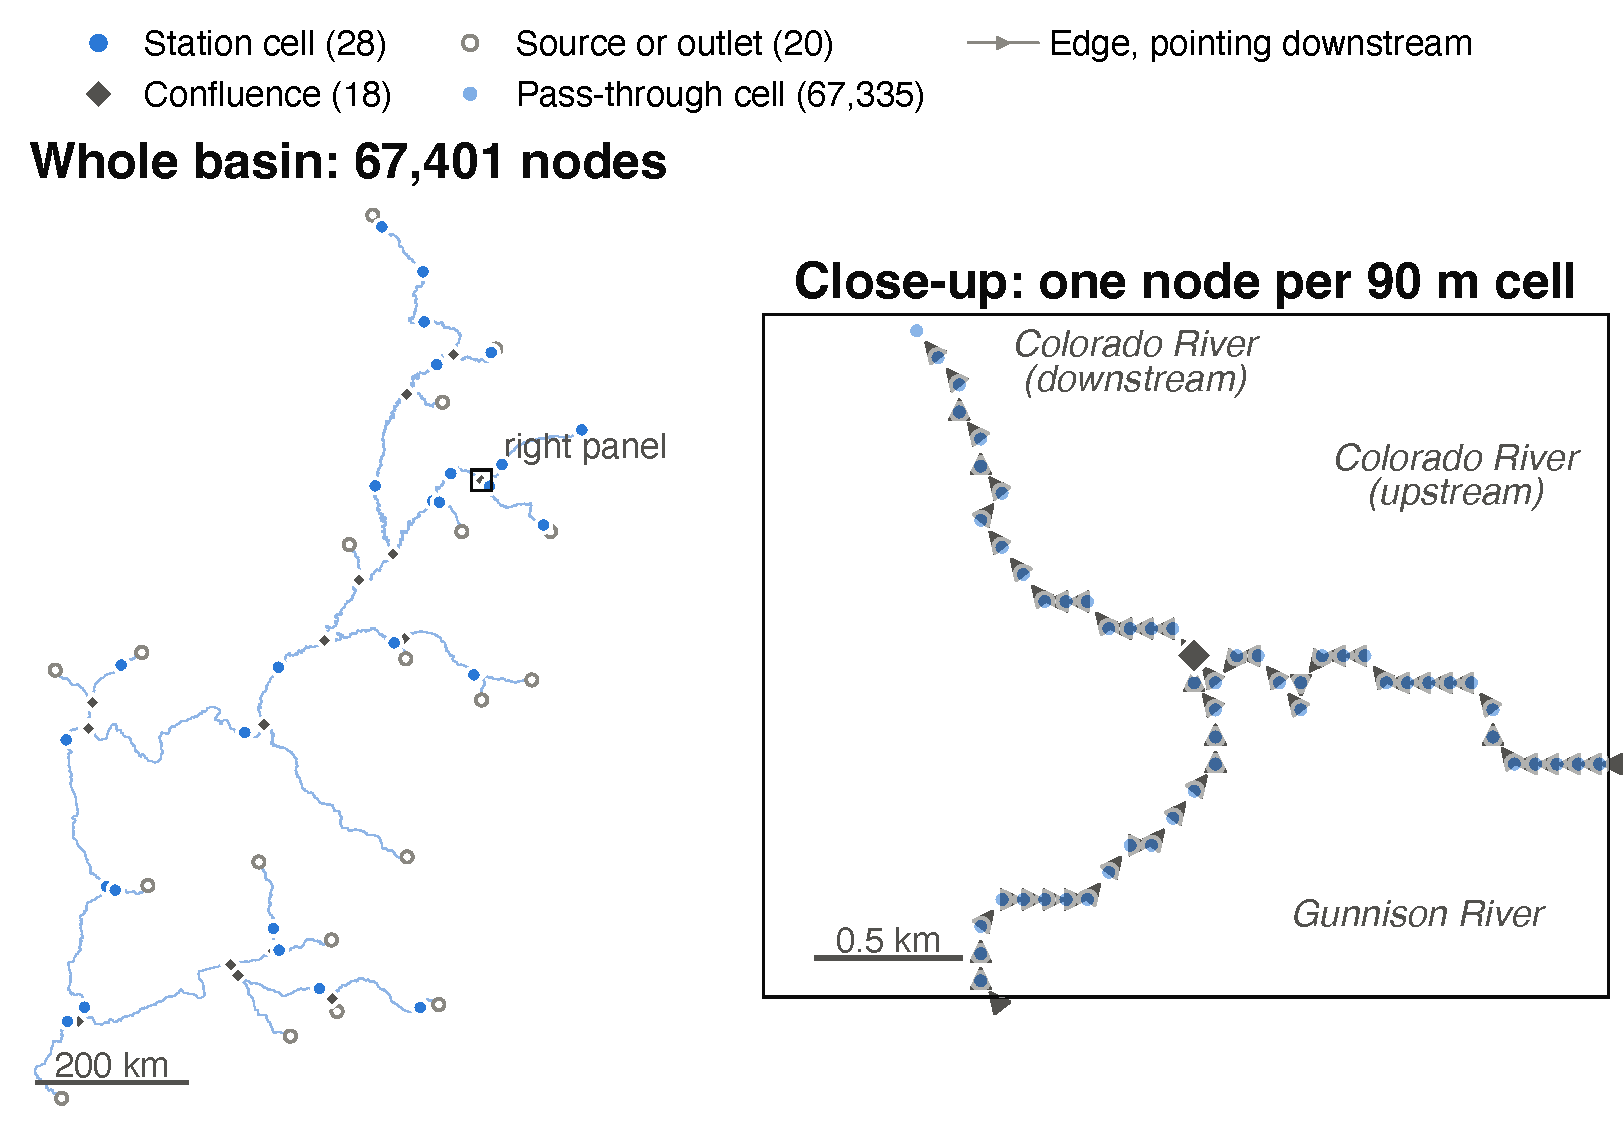
\includegraphics[width=0.788\linewidth]{figures/poster_6_uncompressed.pdf}
    \end{figure}
    \begin{figure}
      \centering
      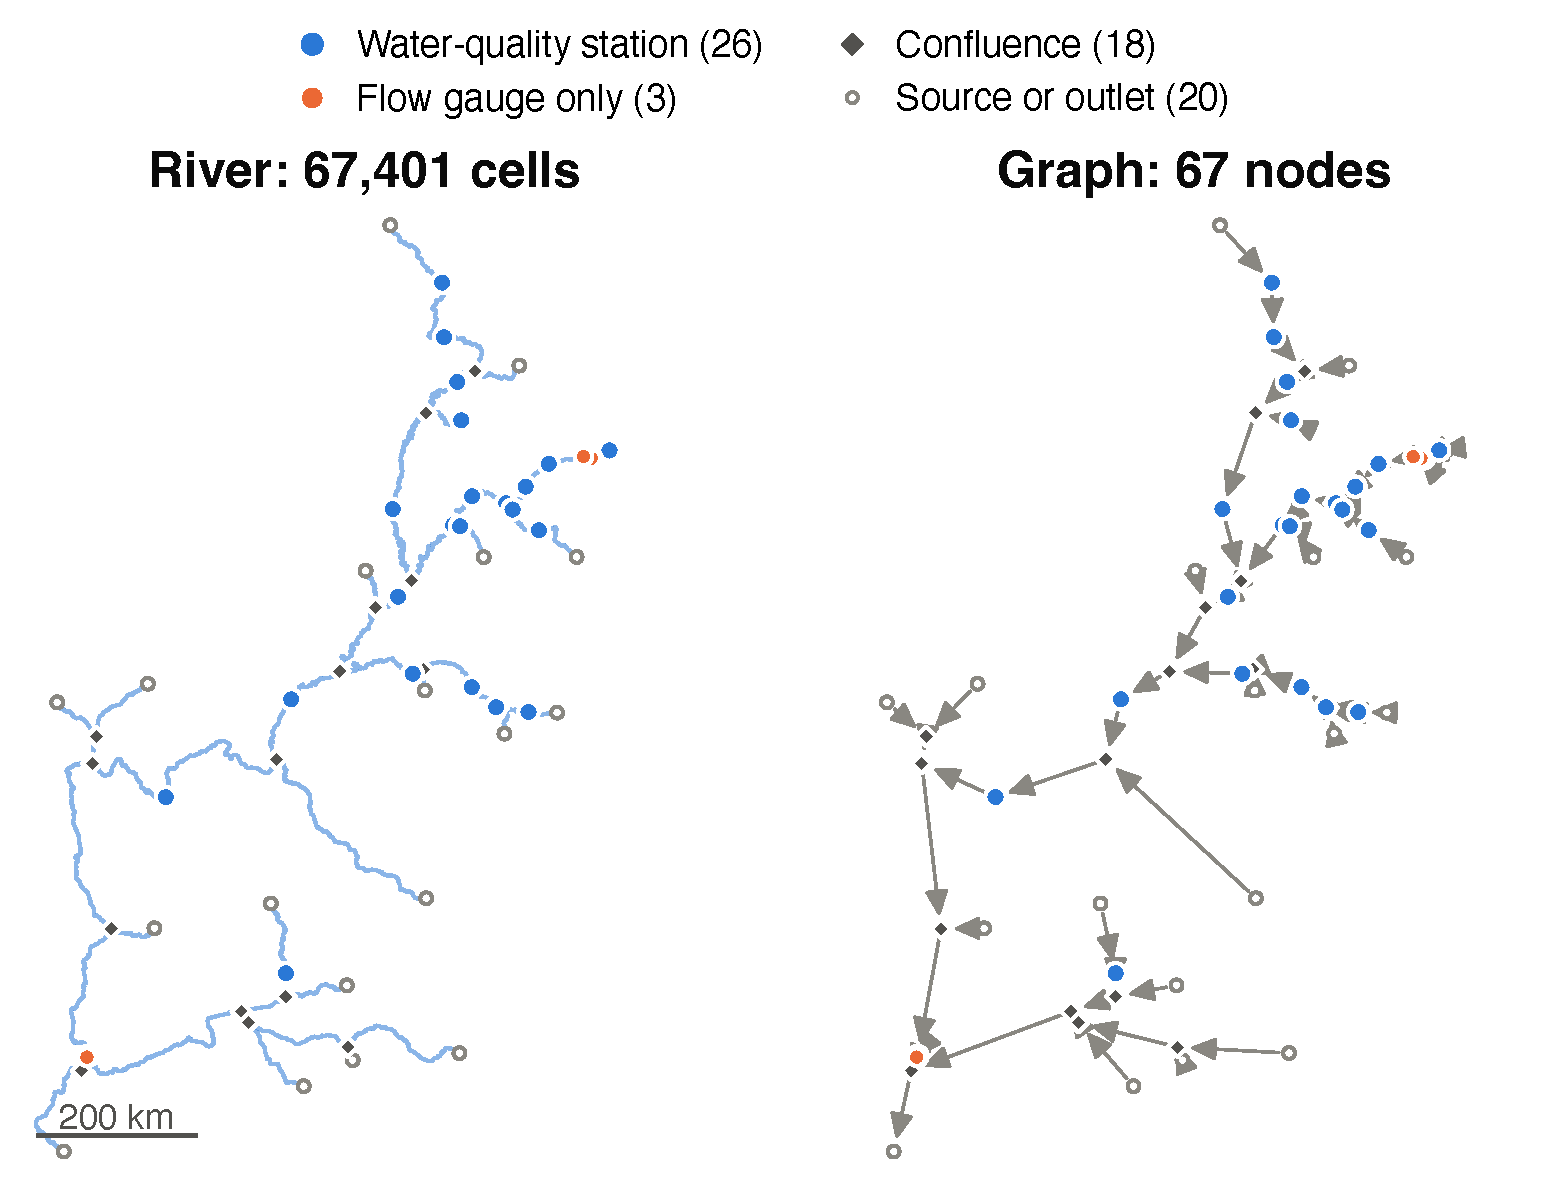
\includegraphics[width=0.788\linewidth]{figures/poster_4_graph.pdf}
    \end{figure}
    \begin{figure}
      \centering
      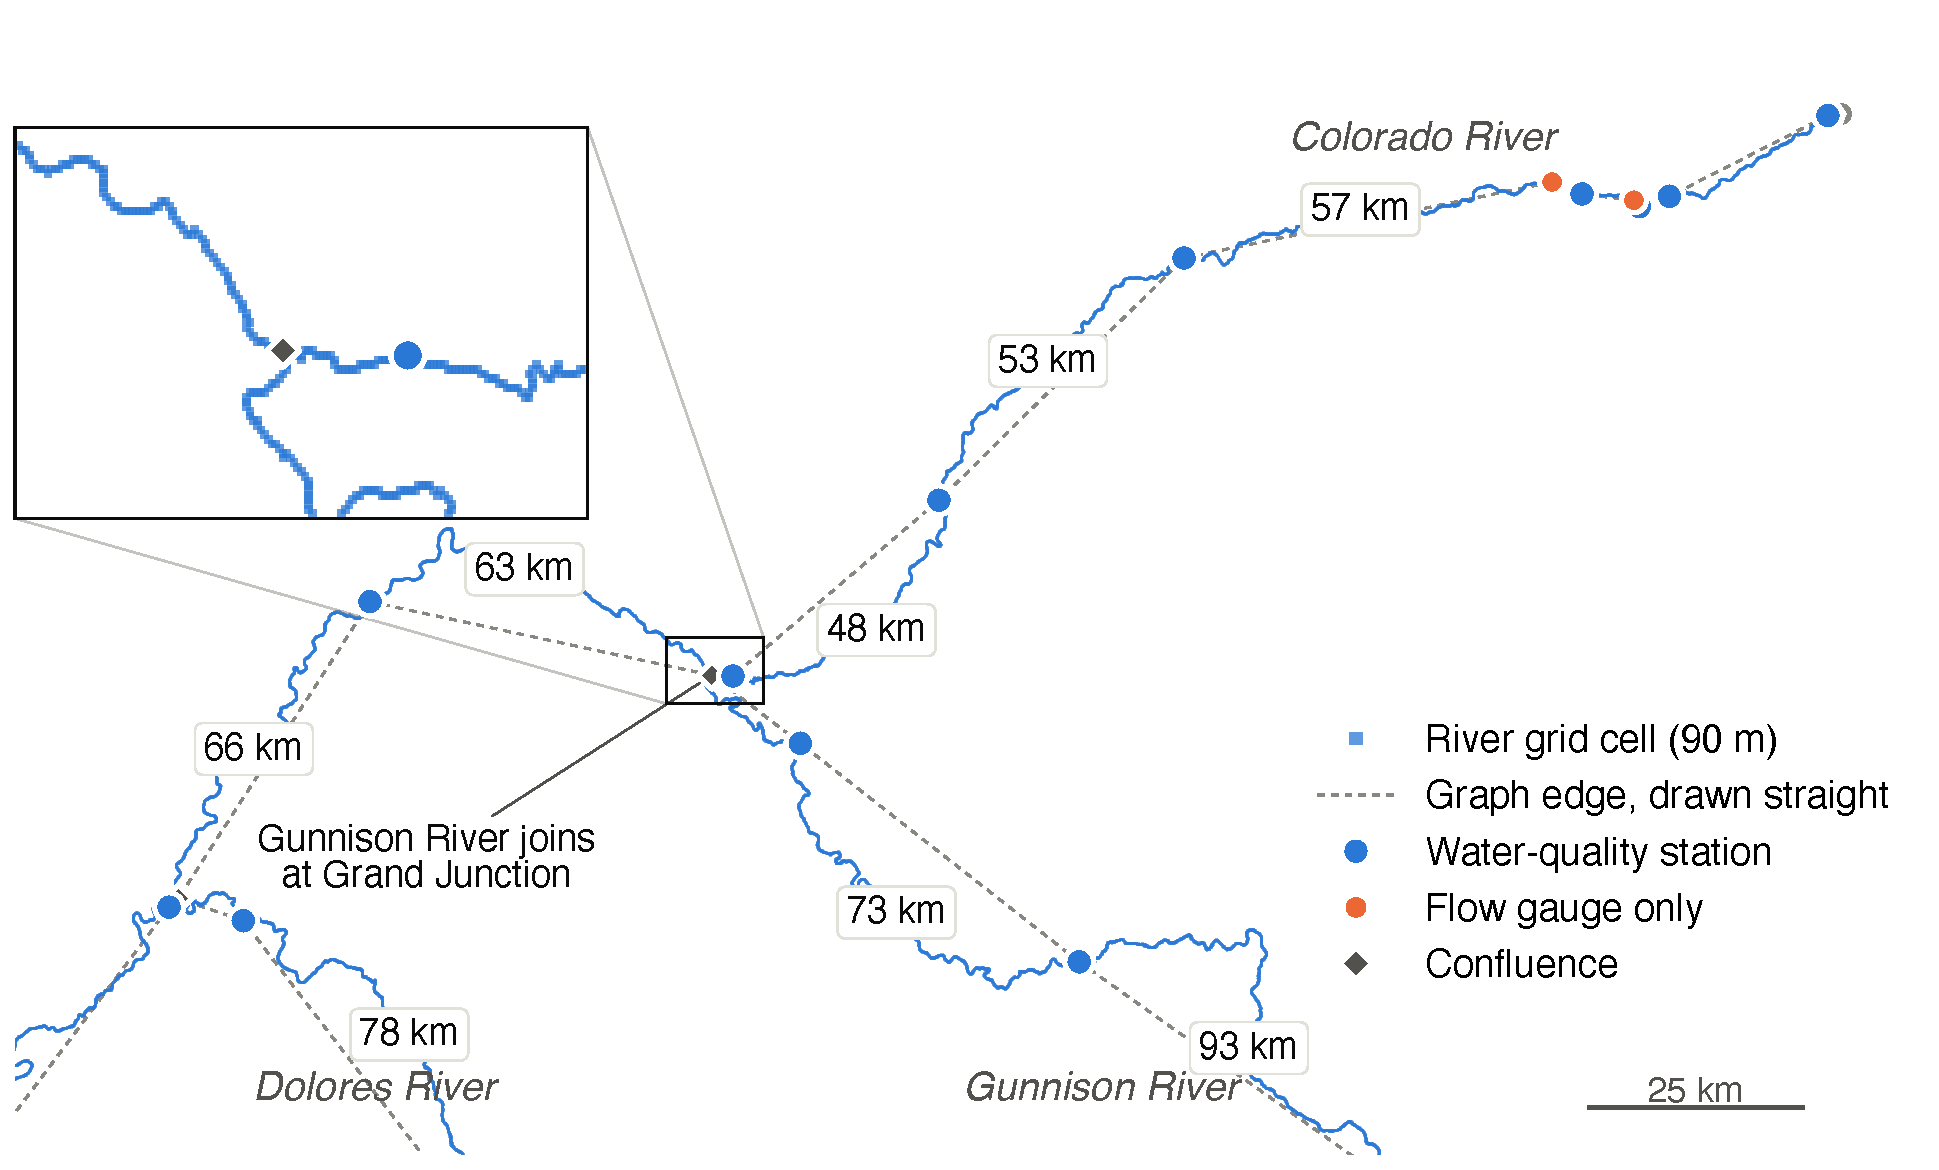
\includegraphics[width=0.788\linewidth]{figures/poster_5_zoom.pdf}
    \end{figure}
  \end{block}

\end{column}

\separatorcolumn

% ===================================================================== column 2
\begin{column}{\colwidth}

  \begin{block}{Graph-Laplacian model}
    For station $i$ and hour $t$, $\hat y_{it} = \beta_0 + z_{it}^\top\beta + g_i$: seasonal and
    daily cycles, other sensor readings and static river attributes $z_{it}$, plus a station
    offset $g_i$ that is smooth along the river:
    \[
      \min_{\beta,\,g}\; \sum_{i}\frac{1}{n_i}\sum_t \bigl(y_{it}-\beta_0-z_{it}^\top\beta-g_i\bigr)^2
      + \lambda_\beta\lVert\beta\rVert^2 + \lambda \sum_{(i,j)} w_{ij}(g_i-g_j)^2 .
    \]
    \textbf{Kron reduction} \cite{dorfler2013,kron1939,schur1917} removes the non-station nodes exactly, leaving a
    $26\times26$ Laplacian. A held-out station's offset is \textbf{interpolated from its
    neighbours along the river}. Evaluation: leave one station out, with all tuning in an inner
    leave-one-out, against six standard models.
  \end{block}

  \begin{block}{Results: model comparison}
    \begin{figure}
      \centering
      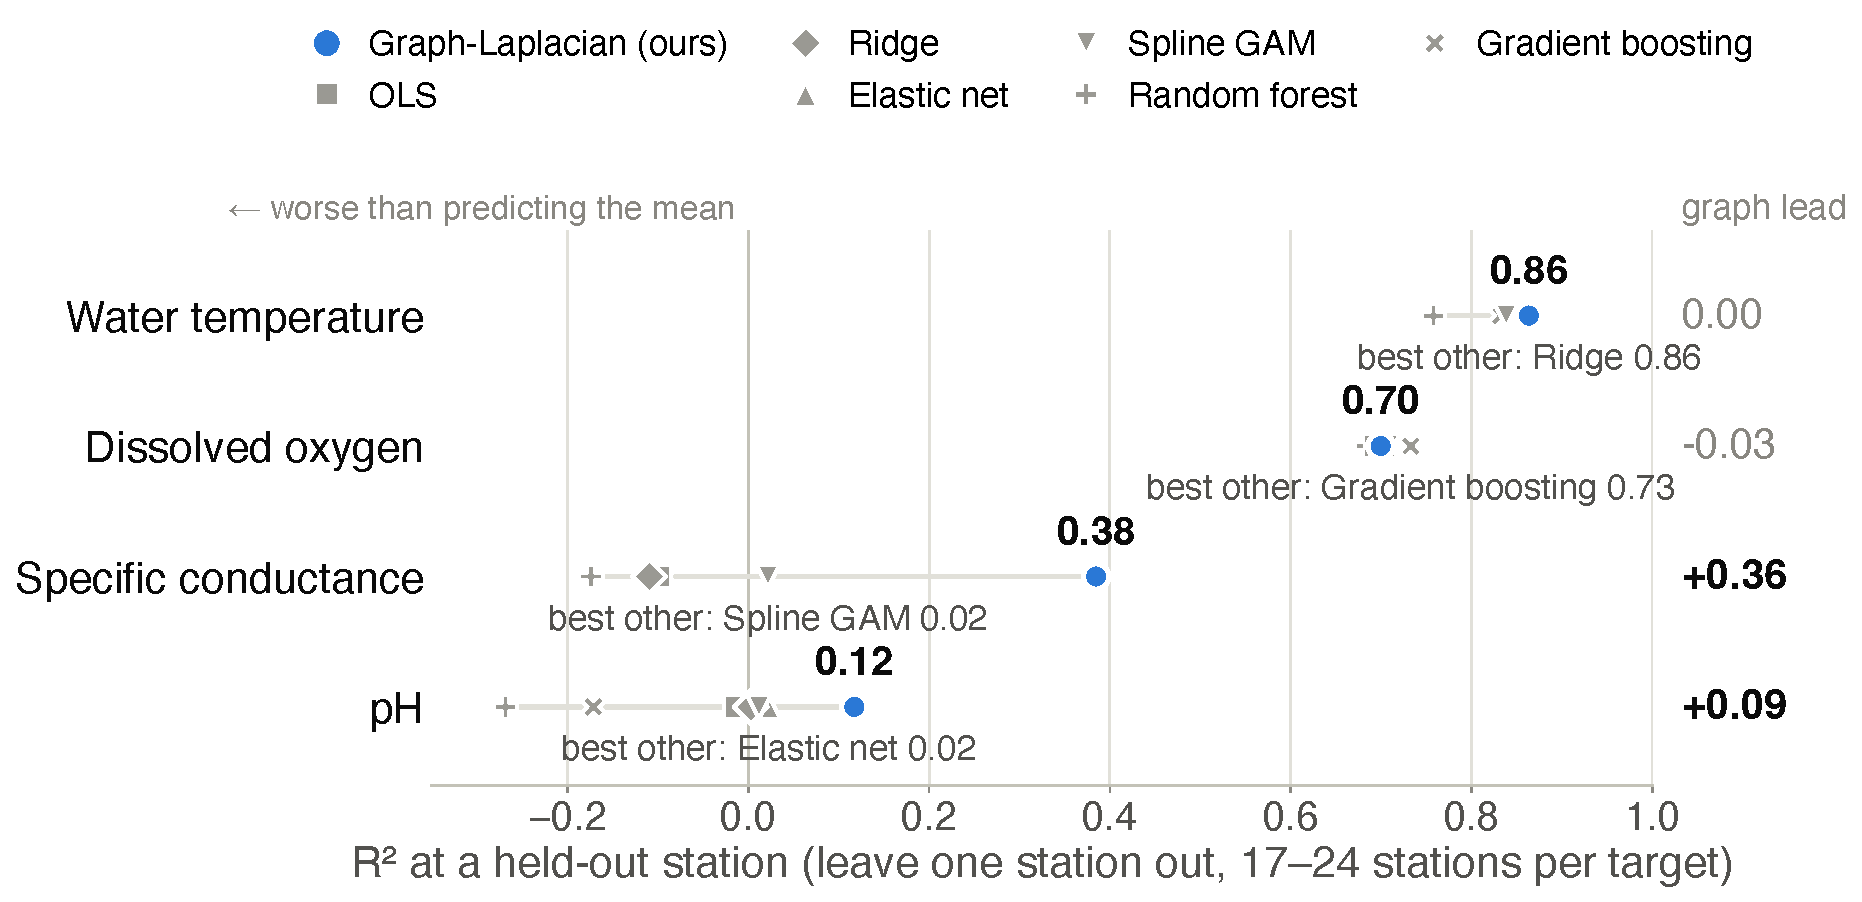
\includegraphics[width=\linewidth]{figures/poster_1_models.pdf}
    \end{figure}
  \end{block}

  \begin{block}{Ablation: what each input contributes}
    Change in the graph model's $R^2$ when one input is removed. Large negative values mark
    inputs nothing else can replace.
    \begin{table}
      \centering
      \begin{tabular}{l c c c c}
        \toprule
        \textbf{Input removed} & \textbf{Water temp.} & \textbf{DO} & \textbf{Spec.\ cond.} & \textbf{pH} \\
        \midrule
        \emph{Full-model $R^2$} & \emph{0.860} & \emph{0.722} & \emph{0.315} & \emph{0.131} \\
        \midrule
        Graph term           & 0.000      & $-$0.008 & $\mathbf{-0.449}$ & $\mathbf{-0.109}$ \\
        Annual cycle         & $\mathbf{-0.721}$ & $-$0.010 & $-$0.107 & $-$0.035 \\
        Daily cycle          & $-$0.009   & $-$0.116 & $+$0.003 & $-$0.043 \\
        Water temperature    & --         & $\mathbf{-0.211}$ & $+$0.025 & -- \\
        Specific conductance & $-$0.002   & $-$0.004 & --       & $-$0.006 \\
        Elevation            & $-$0.030   & $-$0.032 & $-$0.042 & 0.000 \\
        Log upstream area    & $-$0.006   & $-$0.021 & $+$0.078 & 0.000 \\
        Log width            & $+$0.002   & $+$0.004 & $+$0.030 & $+$0.004 \\
        Local slope          & $-$0.039   & $-$0.006 & $-$0.150 & $-$0.026 \\
        \bottomrule
      \end{tabular}
    \end{table}
    The \textbf{graph term} matters most for salinity and pH; water temperature is
    \textbf{seasonality}, and DO follows water temperature and the daily cycle.
  \end{block}

  \begin{block}{How local is the network signal?}
    \begin{figure}
      \centering
      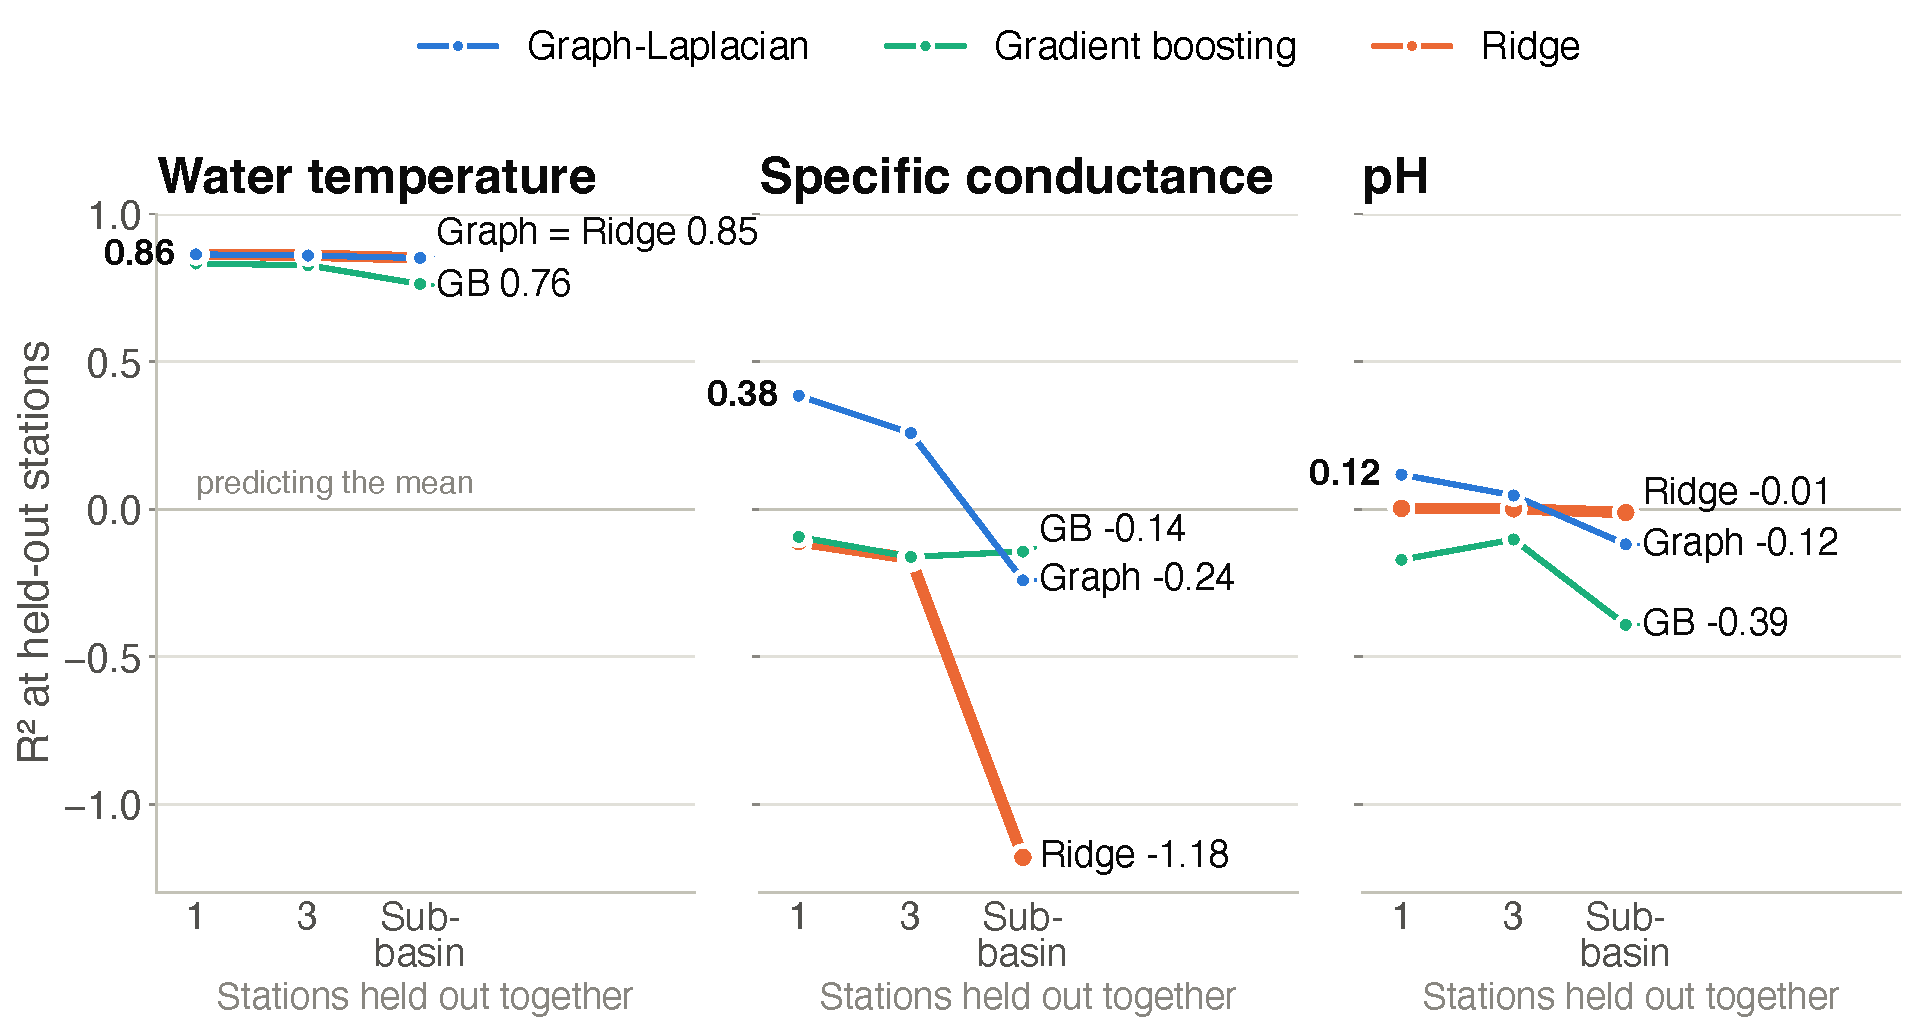
\includegraphics[width=\linewidth]{figures/poster_2_splits.pdf}
    \end{figure}
  \end{block}

\end{column}

\separatorcolumn

% ===================================================================== column 3
\begin{column}{\colwidth}

  \begin{block}{Where the network helps}
    \begin{figure}
      \centering
      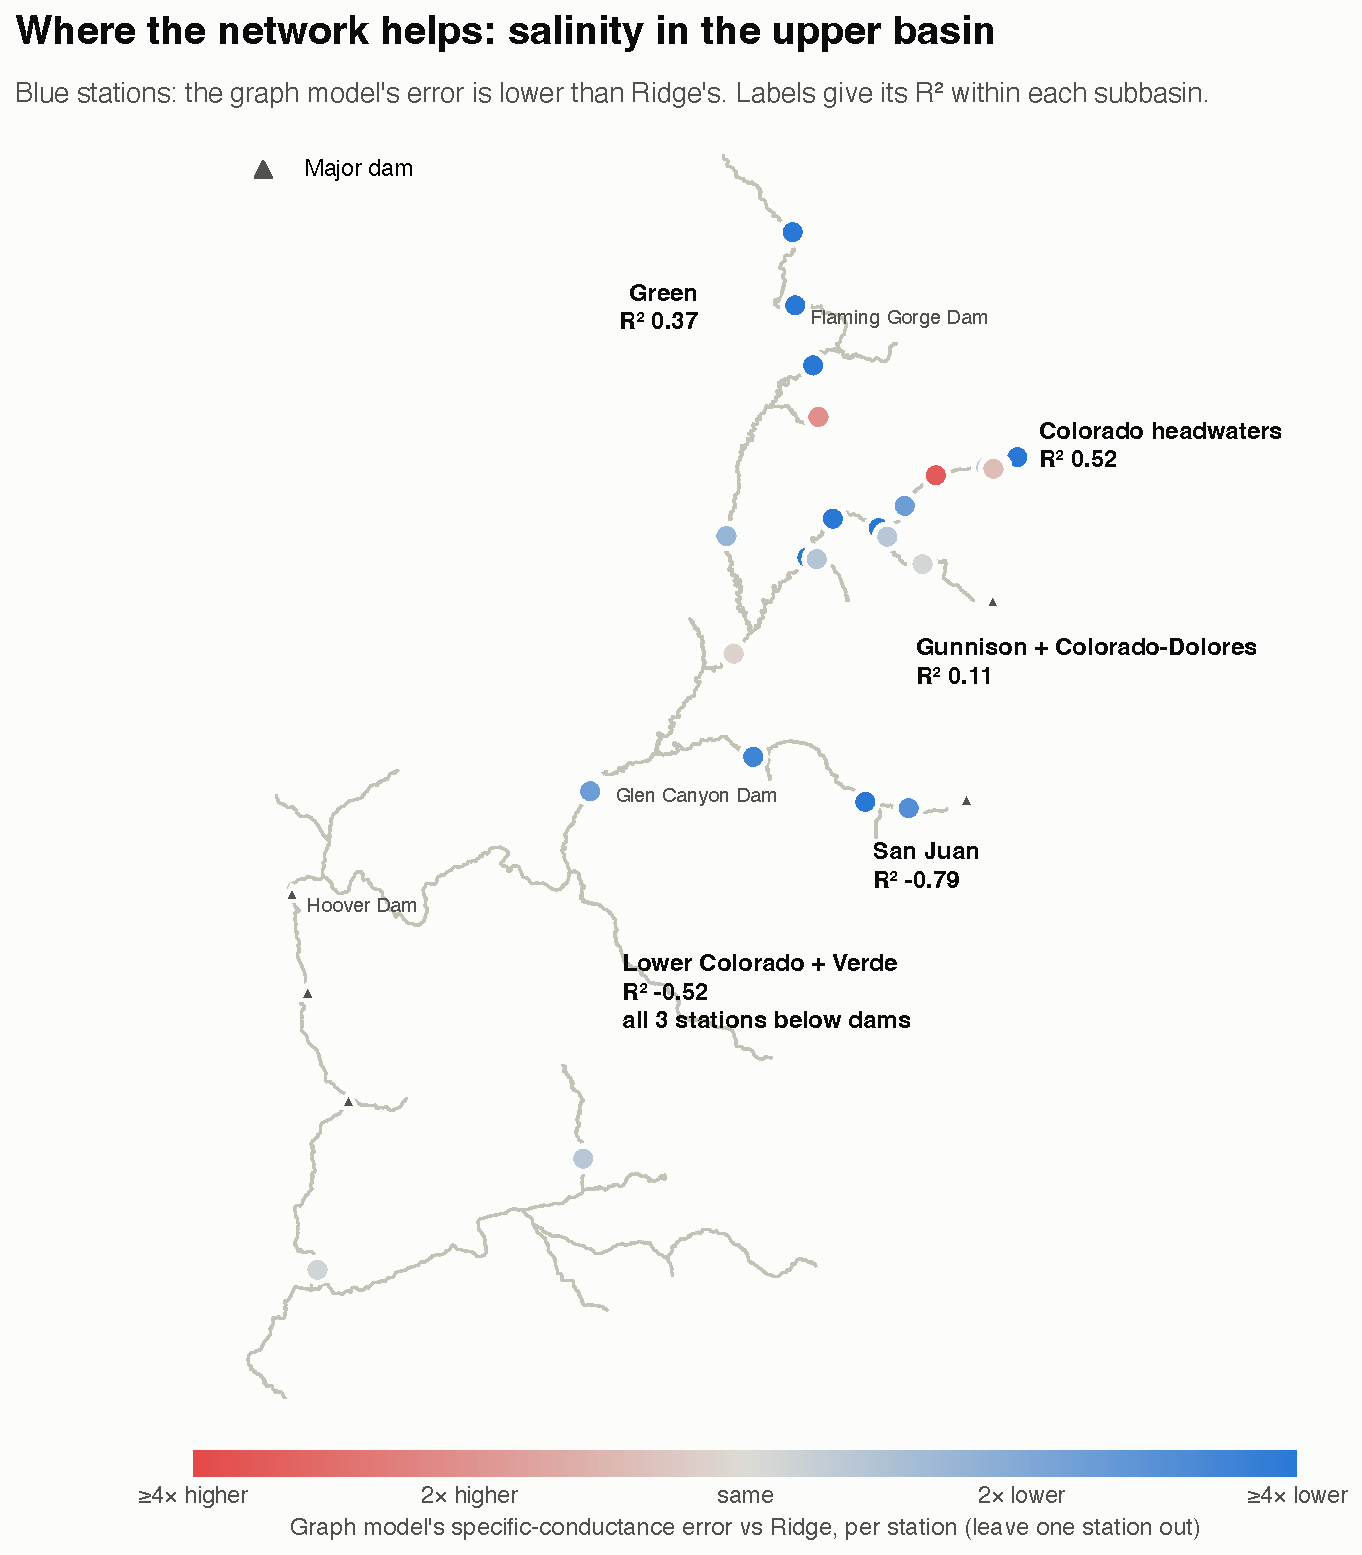
\includegraphics[width=0.78\linewidth]{figures/poster_3_map.pdf}
    \end{figure}
  \end{block}

  \begin{alertblock}{Conclusions}
    \begin{itemize}
      \item A river-network smoothness term predicts \textbf{specific conductance}
            ($R^2$ 0.38 vs 0.02 for the best other model) and \textbf{pH} (0.12 vs 0.02) at
            unseen stations.
      \item Water temperature and DO are driven by season and time of day; the network adds
            nothing there.
      \item The gain comes from \textbf{nearby stations on the same river}: it fades when a whole
            subbasin is held out, and is weakest below the large dams of the lower basin.
    \end{itemize}
  \end{alertblock}

  \begin{block}{References}
    \nocite{*}
    \footnotesize{\bibliographystyle{plain}\bibliography{poster}}
  \end{block}

\end{column}

\separatorcolumn
\end{columns}
\end{frame}

\end{document}
